\chapter{Experiments}
%TODO: explain statistical method: precission, recall, f1, density

Sensitivity and specificity are statistical measures of the performance of a binary classification test, also known in statistics as classification function:

  Sensitivity (also called the true positive rate, or the recall in some fields) measures the proportion of positives that are correctly identified as such (e.g., the percentage of sick people who are correctly identified as having the condition).
    Specificity (also called the true negative rate) measures the proportion of negatives that are correctly identified as such (e.g., the percentage of healthy people who are correctly identified as not having the condition).


    
For the final quantitative evaluation of our experiments we make use of the F1 measure. This measure is often used in determining the performance of  classification tasks in machine learning. To compute its score, this measure takes into account both, the precission and the recall of the test. 
 The exact definition of the F1 measure is given in equation $\ref{eq:f1_score}$.
\begin{equation}
F_1 = 2 \left( \frac{\text{preccision} \times \text{recall}}{\text{preccision} +\text{recall}} \right)
\label{eq:f1_score}
\end{equation}  
The F1 score can be interpreted as a normalized weighted average of the precision and recall test performances. The best possible F1 score is equals 1 and its worst value is 0.
    
\begin{table}[]
\centering
\begin{tabular}{l|l|l|}
\cline{2-3}
 & \begin{tabular}[c]{@{}l@{}}Prediction\\ Positive\end{tabular} & \begin{tabular}[c]{@{}l@{}}Prediction\\ Negative\end{tabular} \\ \hline
\multicolumn{1}{|l|}{\begin{tabular}[c]{@{}l@{}}Condition\\ Positive\end{tabular}} & \cellcolor[HTML]{34FF34}{\color[HTML]{000000} True Positive} & \cellcolor[HTML]{CB0000}False Negative \\ \hline
\multicolumn{1}{|l|}{\begin{tabular}[c]{@{}l@{}}Condiation\\ Negative\end{tabular}} & \cellcolor[HTML]{CB0000}{\color[HTML]{000000} False Positive} & \cellcolor[HTML]{34FF34}True Negative \\ \hline
\end{tabular}
\caption[Prediction and Sensivity]{My caption}
\label{tab:prediction_sensitivity}
\end{table}

\section{Datasets}
\label{sec:datasets}
make table similar to github redme about dataset
display first,center and last frame per dataset

\section{Parameterspace Exploration}
\subsection{Influence of $\lambda$}

\begin{figure}[H]
\centering
\begin{tikzpicture}[trim axis left]
\begin{axis}[
  axis x line=center,
  axis y line=center,
  grid=both,
  xtick={-1,...,10},
  ytick={-1,...,10},
  xlabel={$x$},
  ylabel={$e^{-\lambda d}$},
  xlabel style={below right},
  ylabel style={above left},
  no markers,
  xmin=-0.5,
  xmax=1.5,
  ymin=-1.5,
  ymax=1.5]
\addplot +[thick, domain=0:10] {exp(-x)};
\end{axis}
\end{tikzpicture}
\caption[Affinity Function]{A plot of the affinity transformation function. We observe that the smaller the $\lambda$ paramter gets, the larger the affinities become and wise versa.}
\label{fig:exp_effect_lambda}
\end{figure}


\begin{figure}[H]
\begin{center}

\subfigure[$\lambda = 1$]{
   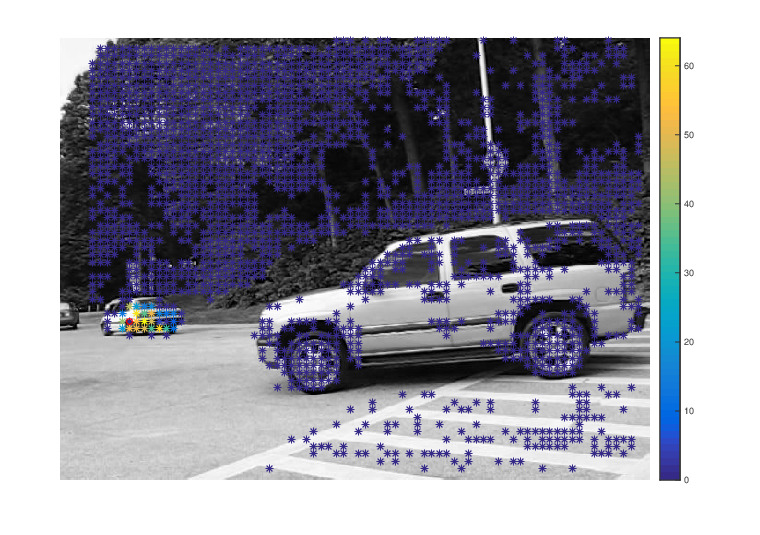
\includegraphics[width=0.48\linewidth] {evaluation/effect_of_lambda/cars_lambda_1}
   \label{fig:cars_eff_lam_a}
}
\subfigure[$\lambda = 0.1$]{
   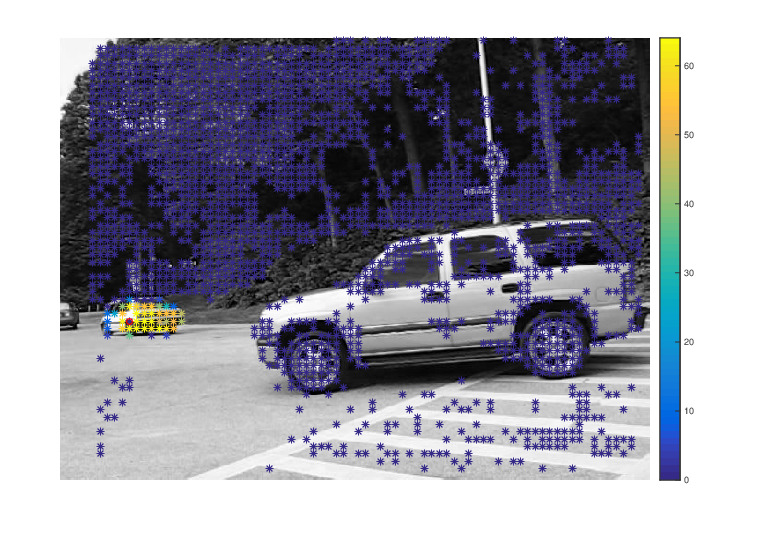
\includegraphics[width=0.48\linewidth] {evaluation/effect_of_lambda/cars_lambda_0_1}
   \label{fig:cars_eff_lam_b}
}
~
\subfigure[$\lambda = 0.01$]{
   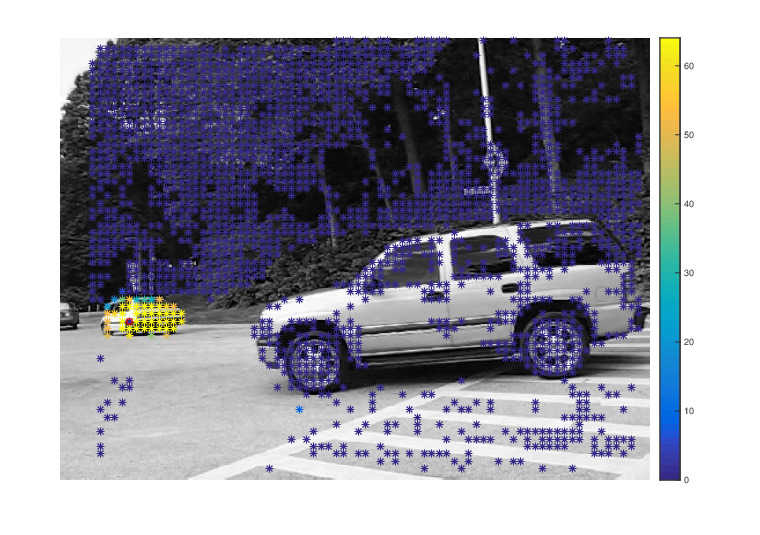
\includegraphics[width=0.48\linewidth] {evaluation/effect_of_lambda/cars_lambda_0_01}
   \label{fig:cars_eff_lam_b}
}
\subfigure[$\lambda = 0.001$]{
   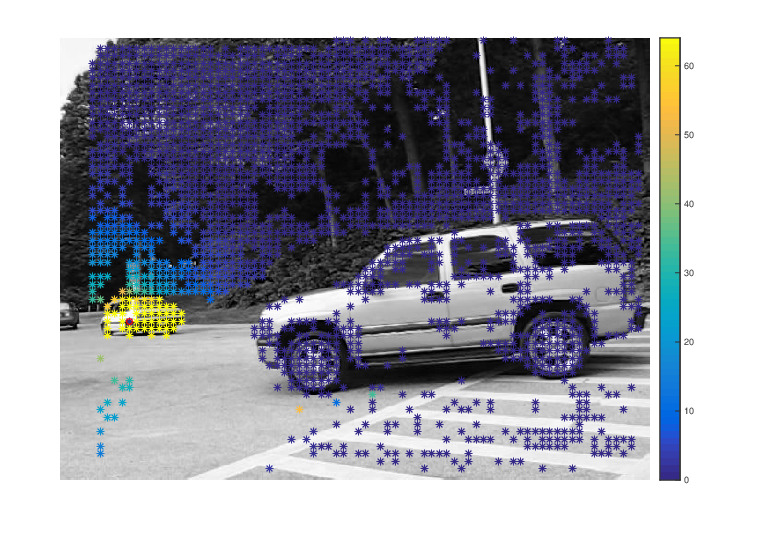
\includegraphics[width=0.48\linewidth] {evaluation/effect_of_lambda/cars_lambda_0_001}
   \label{fig:cars_eff_lam_b}   
}
\end{center}
\caption[Influence of Lambda Parameter]{Illustration of the influence of the $\lambda$ parameter used for computing trajectory affinities. A plot of the affinity transformation function is shown in figure $\ref{fig:exp_effect_lambda}$. }
\label{fig:cars_effect_of_lambda}
\end{figure}

\section{Qualitative Evaluation}
mention available pipeline levels and their main parameters again
tracking candidates

\section{Quantitative Evaluation}


%TODO: statistics: performance of selected set of methods applied on all datasets: HS_PD_SC, LDOF_PD_SC (classic), LDOF_PED_MC, LDOF_SD, LDOF_SED, SRSF_PED, SRSF_SED
%TODO: statistics: influence of lambda using LDOF_PD
%TODO: statistics: LDOF_PED_SC vs LDOF_PD_SC
%TODO: statistics: LDOF_PED_SC vs LDOF_PED_SC
%TODO: statistics: LDOF_PD_MC vs LDOF_SD
%TODO: statistics: LDOF_PED_MC vs LDOF_SED
%TODO: statistics: best case - tweak paras for a dataset.

method comparison, given a fixed number of clusters


\begin{table}[H]
\centering
\begin{tabular}{|l|l|r|l|l|}
\hline
\multicolumn{5}{|c|}{Comparision bonn chairs dataset using 6 clusters}                        \\ \hline
              & \textbf{Density} & \textbf{Precission} & \textbf{Recall} & \textbf{F1 Score} \\ \hline
LDOF PD SC & 0.43685 & 86.2087 \%   & 76.607 \%     & 81.1247 \%  \\ \hline
LDOF PD MC & 0.43685 & 86.4193 \%   & 76.1967 \%     & 80.9867 \%  \\ \hline
LDOF PED SC & 0.37174 & 95.0959 \%   & 78.1937 \%     & 85.8205 \%  \\ \hline
LDOF PED MC & 0.37174 & 83.3878 \%   & 91.4203 \%     & 87.2195 \%  \\ \hline              
LDOF SD & 0.43848 & 74.7623 \%   & 96.4264 \%     & 84.2235 \%  \\ \hline
\end{tabular}
\caption[Cars Dataset]{My caption}
\label{tab:eval_bonn_chairs}
\end{table}


\begin{figure}[H]
\begin{center}
\subfigure[GT]{
   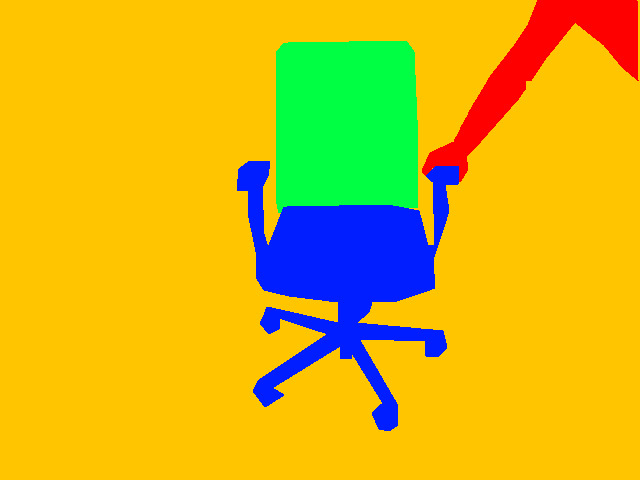
\includegraphics[width=0.48\linewidth] {evaluation/bonn_chairs/gt_20}
   \label{fig:bonn_chairs_a}
}
~
\subfigure[LDOF PD SC]{
   \includegraphics[width=0.48\linewidth] {evaluation/bonn_chairs/ldof_pd_sc}
   \label{fig:bonn_chairs_b}
}
\subfigure[LDOF PD MC]{
   \includegraphics[width=0.48\linewidth] {evaluation/bonn_chairs/ldof_pd_mc}
   \label{fig:bonn_chairs_c}
}
~
\subfigure[LDOF PED SC]{
   \includegraphics[width=0.48\linewidth] {evaluation/bonn_chairs/ldof_ped_sc}
   \label{fig:bonn_chairs_d}
}
\subfigure[LDOF PED MC]{
   \includegraphics[width=0.48\linewidth] {evaluation/bonn_chairs/ldof_ped_mc}
   \label{fig:bonn_chairs_e}
}
\end{center}
\caption[Evaluation Bonn Chairs]{pew}
\label{fig:eval_bonn_chairs}
\end{figure}



Fragmentation: 0.66667


\begin{table}[H]
\centering
\begin{tabular}{|l|l|r|l|l|}
\hline
\multicolumn{5}{|c|}{Comparision cars dataset 3 clusters}                        \\ \hline
              & \textbf{Density} & \textbf{Precission} & \textbf{Recall} & \textbf{F1 Score} \\ \hline
LDOF PD SC & 0.66829 & 91.0544 \%   & 89.8432 \%     & 90.4447 \%  \\ \hline
LDOF PD MC & 0.66829 & 91.0502 \%   & 88.9107 \%     & 89.9677 \%  \\ \hline              
LDOF SD & 0.69987 & 79.2541 \%   & 92.709 \%     & 85.4551 \%  \\ \hline
\end{tabular}
\caption[Cars Dataset]{My caption}
\label{tab:cars_ldof_quality}
\end{table}

\begin{figure}[H]
\begin{center}

\subfigure[GT]{
   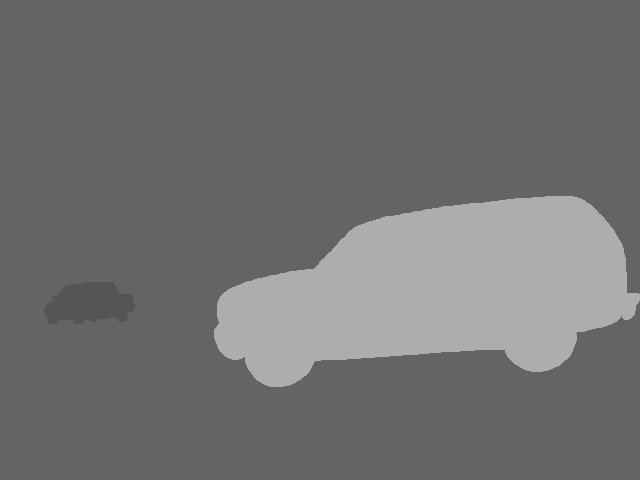
\includegraphics[width=0.48\linewidth] {evaluation/method_2d_ds/gt_1}
   \label{fig:cars_a}
}
\subfigure[LDOF PD SC]{
   \includegraphics[width=0.48\linewidth] {evaluation/method_2d_ds/ldof_pd_sc}
   \label{fig:cars_b}
}
~
\subfigure[LDOF PD MC]{
   \includegraphics[width=0.48\linewidth] {evaluation/method_2d_ds/ldof_pd_mc}
   \label{fig:cars_c}
}
\subfigure[LDOF SD]{
   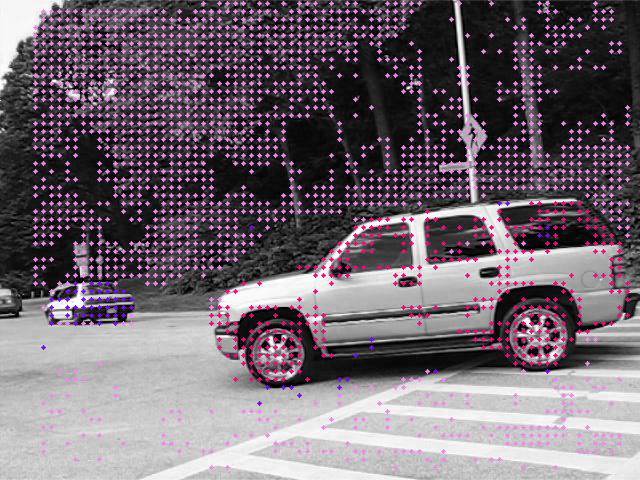
\includegraphics[width=0.48\linewidth] {evaluation/method_2d_ds/ldof_sd}
   \label{fig:cars_d}   
}
\end{center}
\caption[Method Comparison]{Visualization of segmentation resulting when running our pipeline on a dataset without depth information.}
\label{fig:cars_dataset}
\end{figure}




dataset: bonn watercan
Fragmentation: 0.66667

\begin{figure}[H]
\begin{center}
\subfigure[GT Waterbox Frame 4]{
   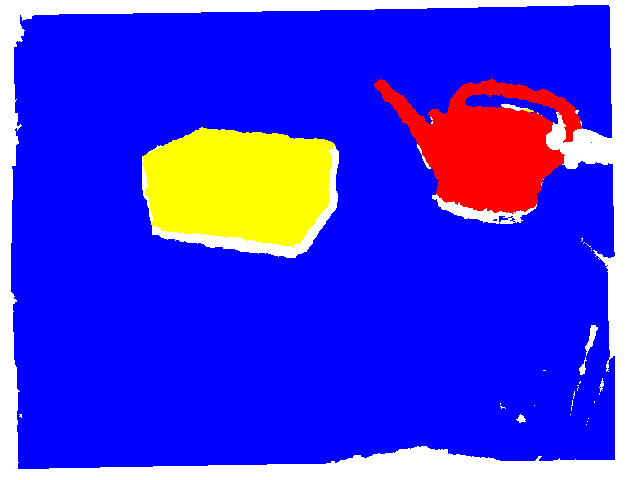
\includegraphics[width=0.7\linewidth] {evaluation/meth_cmp_bonn_wc/gt_4}
   \label{fig:bonn_gieskanne_gt}
}
~
\subfigure[LDOF PED SC]{
   \includegraphics[width=0.48\linewidth] {evaluation/meth_cmp_bonn_wc/ldof_ped_sc}
   \label{fig:bonn_wc_a}
}
\subfigure[LDOF PED SC]{
   \includegraphics[width=0.48\linewidth] {evaluation/meth_cmp_bonn_wc/ldof_ped_mc}
   \label{fig:bonn_wc_b}
}
~
\subfigure[SRSF PED SC]{
   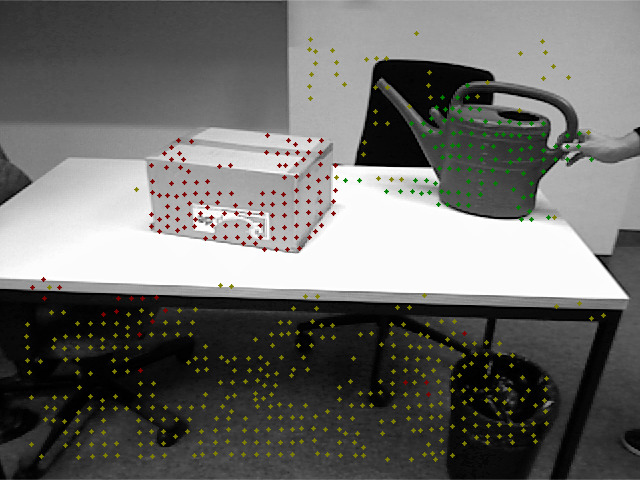
\includegraphics[width=0.48\linewidth] {evaluation/meth_cmp_bonn_wc/srsf_ped_sc}
   \label{fig:bonn_wc_c}
}
\subfigure[SRSF PED MC]{
   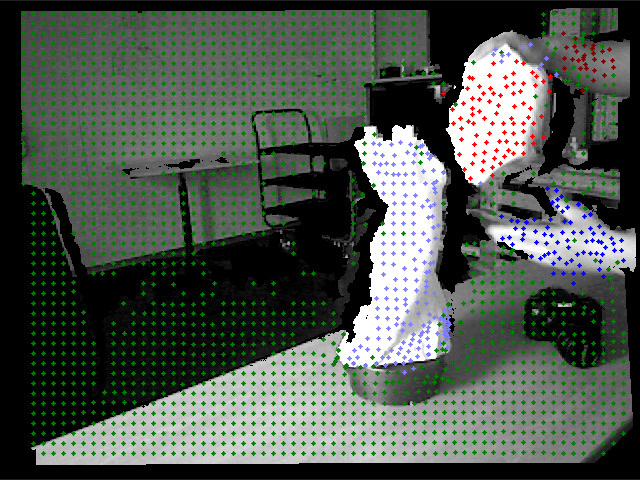
\includegraphics[width=0.48\linewidth] {evaluation/meth_cmp_bonn_wc/srsf_ped_mc}
   \label{fig:bonn_wc_d}   
}
\end{center}
\caption[Method Comparison]{Visualization of merged segmentations when comparing various methods}
\label{fig:bonn_watercan_method_cmp}
\end{figure}

\begin{figure}[H]
\begin{center}
\subfigure[LDOF PD SC]{
   \includegraphics[width=0.48\linewidth] {evaluation/meth_cmp_bonn_wc/ldof_pd_sc}
   \label{fig:bonn_wc_ed}
}
\subfigure[LDOF PD MC]{
   \includegraphics[width=0.48\linewidth] {evaluation/meth_cmp_bonn_wc/ldof_pd_mc}
   \label{fig:bonn_wc_f}   
}
\end{center}
\caption[Method Comparison 2]{Visualization of merged segmentations when comparing various methods}
\label{fig:bonn_watercan_method_cmp_2}
\end{figure}


\begin{table}[]
\centering
\begin{tabular}{|l|l|r|l|l|}
\hline
\multicolumn{5}{|c|}{Method Comparison, 12 fixed Clusters, Bonn Watercan}                        \\ \hline
              & \textbf{Density} & \textbf{Precission} & \textbf{Recall} & \textbf{F1 Score} \\ \hline
LDOF PD SC * & 0.44434 & 72.783 \%   & 66.1853 \%     & 69.3275 \%  \\ \hline
LDOF PD MC * & 0.44434 & 34.1727 \%   & 45.6731 \%     & 39.0947 \%  \\ \hline              
LDOF PED SC * & 0.43522 & 94.2955 \%   & 58.2015 \%     & 71.9770 \%  \\ \hline
LDOF PED MC * & 0.43522 & 64.4977 \%   & 81.0601 \%     & 71.8366 \%  \\ \hline
LDOF SD KL & 0.21094 & 84.4582 \%   & 70 \%     & 75.8336 \%  \\ \hline
LDOF SED KL & 0.21094 & 84.4582 \%   & 70 \%     & 75.8336 \%  \\ \hline
SRSF PD SC & 0.21094 & 84.4582 \%   & 70 \%     & 75.8336 \%  \\ \hline
SRSF PD MC & 0.21094 & 84.4582 \%   & 70 \%     & 75.8336 \%  \\ \hline
SRSF PED SC * & 0.20085 & 83.5144 \%   & 95.7385 \%     & 89.2096 \%  \\ \hline
SRSF PED MC * & 0.19889 & 92.9871 \%   & 70 \%     & 79.8725 \%  \\ \hline
SRSF SD KL & 0.21094 & 84.4582 \%   & 70 \%     & 75.8336 \%  \\ \hline
SRSF SED KL & 0.21094 & 84.4582 \%   & 70 \%     & 75.8336 \%  \\ \hline
\end{tabular}
\caption[Method Comparision Bonn Watercan]{My caption}
\label{tab:bonn_wc_methods}
\end{table}


explain the assumption of the datasets
explain what kind of segmentations have been generated and evaluated.







parameterspace exploration
running different similarity tasks




